% This is "sig-alternate.tex" V2.1 April 2013
% This file should be compiled with V2.5 of "sig-alternate.cls" May 2012
%
% This example file demonstrates the use of the 'sig-alternate.cls'
% V2.5 LaTeX2e document class file. It is for those submitting
% articles to ACM Conference Proceedings WHO DO NOT WISH TO
% STRICTLY ADHERE TO THE SIGS (PUBS-BOARD-ENDORSED) STYLE.
% The 'sig-alternate.cls' file will produce a similar-looking,
% albeit, 'tighter' paper resulting in, invariably, fewer pages.
%
% ----------------------------------------------------------------------------------------------------------------
% This .tex file (and associated .cls V2.5) produces:
%       1) The Permission Statement
%       2) The Conference (location) Info information
%       3) The Copyright Line with ACM data
%       4) NO page numbers
%
% as against the acm_proc_article-sp.cls file which
% DOES NOT produce 1) thru' 3) above.
%
% Using 'sig-alternate.cls' you have control, however, from within
% the source .tex file, over both the CopyrightYear
% (defaulted to 200X) and the ACM Copyright Data
% (defaulted to X-XXXXX-XX-X/XX/XX).
% e.g.
% \CopyrightYear{2007} will cause 2007 to appear in the copyright line.
% \crdata{0-12345-67-8/90/12} will cause 0-12345-67-8/90/12 to appear in the copyright line.
%
% ---------------------------------------------------------------------------------------------------------------
% This .tex source is an example which *does* use
% the .bib file (from which the .bbl file % is produced).
% REMEMBER HOWEVER: After having produced the .bbl file,
% and prior to final submission, you *NEED* to 'insert'
% your .bbl file into your source .tex file so as to provide
% ONE 'self-contained' source file.
%
% ================= IF YOU HAVE QUESTIONS =======================
% Questions regarding the SIGS styles, SIGS policies and
% procedures, Conferences etc. should be sent to
% Adrienne Griscti (griscti@acm.org)
%
% Technical questions _only_ to
% Gerald Murray (murray@hq.acm.org)
% ===============================================================
%
% For tracking purposes - this is V2.0 - May 2012

\documentclass{sig-alternate-05-2015}

%for the table
\usepackage{booktabs}

%for [H]
\usepackage{float}
\usepackage{graphicx}
\PassOptionsToPackage{hyphens}{url}\usepackage{hyperref}

\usepackage{url}
\newcommand{\textprime}{\ensuremath{'}}
\begin{document}

% Copyright
%\setcopyright{acmcopyright}
%\setcopyright{acmlicensed}
%\setcopyright{rightsretained}
%\setcopyright{usgov}
%\setcopyright{usgovmixed}
%\setcopyright{cagov}
%\setcopyright{cagovmixed}


% DOI
%\doi{10.475/123_4}

% ISBN
%\isbn{123-4567-24-567/08/06}

%Conference
%\conferenceinfo{PLDI '13}{June 16--19, 2013, Seattle, WA, USA}

%\acmPrice{\$15.00}

%
% --- Author Metadata here ---
%\conferenceinfo{WOODSTOCK}{'97 El Paso, Texas USA}
%\CopyrightYear{2007} % Allows default copyright year (20XX) to be over-ridden - IF NEED BE.
%\crdata{0-12345-67-8/90/01}  % Allows default copyright data (0-89791-88-6/97/05) to be over-ridden - IF NEED BE.
% --- End of Author Metadata ---

\title{ Stock Price Prediction Using Twitter}
%\subtitle{[Extended Abstract]
%\titlenote{A full version of this paper is available as
%\textit{Author's Guide to Preparing ACM SIG Proceedings Using
%\LaTeX$2_\epsilon$\ and BibTeX} at
%\texttt{www.acm.org/eaddress.htm}}}
%
% You need the command \numberofauthors to handle the 'placement
% and alignment' of the authors beneath the title.
%
% For aesthetic reasons, we recommend 'three authors at a time'
% i.e. three 'name/affiliation blocks' be placed beneath the title.
%
% NOTE: You are NOT restricted in how many 'rows' of
% "name/affiliations" may appear. We just ask that you restrict
% the number of 'columns' to three.
%
% Because of the available 'opening page real-estate'
% we ask you to refrain from putting more than six authors
% (two rows with three columns) beneath the article title.
% More than six makes the first-page appear very cluttered indeed.
%
% Use the \alignauthor commands to handle the names
% and affiliations for an 'aesthetic maximum' of six authors.
% Add names, affiliations, addresses for
% the seventh etc. author(s) as the argument for the
% \additionalauthors command.
% These 'additional authors' will be output/set for you
% without further effort on your part as the last section in
% the body of your article BEFORE References or any Appendices.

\numberofauthors{4} %  in this sample file, there are a *total*
% of EIGHT authors. SIX appear on the 'first-page' (for formatting
% reasons) and the remaining two appear in the \additionalauthors section.
%
\author{
% You can go ahead and credit any number of authors here,
% e.g. one 'row of three' or two rows (consisting of one row of three
% and a second row of one, two or three).
%
% The command \alignauthor (no curly braces needed) should
% precede each author name, affiliation/snail-mail address and
% e-mail address. Additionally, tag each line of
% affiliation/address with \affaddr, and tag the
% e-mail address with \email.
%
% 1st. author
\alignauthor
Amal Duriseti\\%\titlenote{Dr.~Trovato insisted his name be first.}\\
       \affaddr{904331855}\\
    %   \affaddr{1932 Wallamaloo Lane}\\
      % \affaddr{Los Angeles, California}\\
       \email{aduriseti@gmail.com}
% 2nd. author
\alignauthor
Jonathan Hurwitz\\
       \affaddr{804258351}\\
      % \affaddr{P.O. Box 1212}\\
       %\affaddr{Los Angeles, California}\\
       \email{jdhurwitz@ucla.edu}
% 3rd. author
\alignauthor  Fred Xu\\
       \affaddr{004255573}\\
     %  \affaddr{1 Th{\o}rv{\"a}ld Circle}\\
       %\affaddr{}\\
       \email{xuzeyuanfred@ucla.edu}
\and  % use '\and' if you need 'another row' of author names
% 4th. author
\alignauthor Jerry Chen\\
       \affaddr{804449266}\\
     %  \affaddr{Brookhaven National Lab}\\
      % \affaddr{P.O. Box 5000}\\
       \email{hostmissile@hotmail.com}
}
% There's nothing stopping you putting the seventh, eighth, etc.
% author on the opening page (as the 'third row') but we ask,
% for aesthetic reasons that you place these 'additional authors'

% Just remember to make sure that the TOTAL number of authors
% is the number that will appear on the first page PLUS the
% number that will appear in the \additionalauthors section.

\maketitle

	\maketitle
	\begin{abstract}
		This project aims to predict buy or sell indicators for several large S\&P500 companies based on Twitter data. This is a form of classification rather than regression. The first iteration of our project aimed to predict mood based on tweets, but we pivoted and leveraged learnings from the previously done sentiment analysis work in order to build our stock predictor. Several machine learning models have been tested and compared. We settled on using a feed-forward neural network, or multi-layer perceptron (MLP), to perform the predictions.  
	\end{abstract}
	
	
	\section{Introduction}
	The former goal was to create an aggregate mood detector and predictor by training machine learning models to perform sentiment analysis on tweets. This task implicitly includes building some method of obtaining more data, such as a data crawler. While our models showed reasonably good performance when trained on the twitter sentiment analysis training corpus\footnote{The sentiment analysis corpus contains 1.5M tweets and can be downloaded at \url{http://thinknook.com/twitter-sentiment-analysis-training-corpus-dataset-2012-09-22/}}, we realized that some sort of unsupervised learning would have to be done in order to label future data obtained via the crawler. This motivated us to explore other ways in which we could leverage our previous work but for a task with an easier means of labeling data.
	\subsection{Problem Definition and Formalization}
	Using sentiment to predict buy or sell indicators seemed like a natural progression with an easier way of labeling data. The labeling scheme we chose was to associate each tweet with the corresponding stock price on the day it was tweeted. The crawler pulls tweets and labels each tweet by doing a yahoo finance price lookup. This way, we are able to build an arbitrarily large dataset of labeled tweets in order to better train our models. There is no need for unsupervised learning such as clustering in order to assign class labels.
	\par
	To formalize, the goal of the project was, given a set of tweets about a company (by stock ticker), to predict whether the stock would go up or down on the open of the next trading day by using sentiment analysis.
	\par
	All code for this project can be found here: \url{https://github.com/aduriseti/cs145_project}. All of the work was done in Jupyter notebooks.
	\section{Data Crawler}
	The data crawler performs tweet lookup, preprocessing, and labeling for an arbitrary number of stock tickers or query strings. It is assumed that data for each query will be pulled for each day within the specified date range. 
	\par
	Within the scope of this project, the queries were all stock tickers for several large companies: AAPL, AMZN, SNE, GOOG, NVDA, INTC, HPQ, MSFT, IBM, and TXN. Each of these tickers is given their own thread to perform the lookup, filtering, and labeling. The initial intent was to perform a live lookup on Yahoo finance in order to obtain stock prices for labeling, but there were issues with Yahoo finance historical data. After writing a function to pull data using BeautifulSoup, we decided it would be best to just download local csv files from Yahoo containing the data for each ticker over the desired time range (from min to max date). 
	\par 
	For each day in the date range, the crawler queries twitter and limits the number of tweets pulled via the "max\_tweets" parameter.  Tweets are processed in batches corresponding to each day. Tweets for a specific ticker that were posted on a day in which there is no associated stock price are removed from the set. Duplicates are also removed. Stock price labels are 5-D and consist of the open, high, low, close, and adj close. The intent was to provide the maximum amount of information for us to use in learning algorithm evaluation. Following a successful tweet:label pairing, the crawler writes this to a file along with the date of the tweet and continues.
	\section{Methods Description}
	After obtaining raw data by means of our data crawler, we took the following approach:
	\begin{enumerate}
		\item Preprocess the data via tokenization.
		\item Test various models for sentiment analysis performance on a set of commonly used metrics.
		\item Choose the most effective model and perform hyperparameter tuning on it.
		\item Concurrently test exploratory designs on more complicated RNN-based models, such as the LSTM.
		\item Integrate the most effective model from above steps into the stock prediction task, and use the same classification metrics as before to determine performance.
	\end{enumerate}
	As mentioned, in our case the stock price prediction is a classification task rather than a regression task since we are simply outputting binary results: "expected to go up tomorrow" or "expected to go down tomorrow".
	\section{Sentiment Analysis}
	We trained a variety of classifiers on the Twitter sentiment analysis training corpus. These included random forest, multi-layer perceptron (MLP), and quadratic discriminant analysis. In addition, we tested the RNN-based long short-term memory (LSTM) model. SVM was avoided due to long training time.
	\par
	 The embedding scheme involved using word2vec and a mean aggregation method. The word2vec vectors are trained on the set of aggregated tweets created by the crawler. For each word within a tweet, we check to see if it is in the trained word2vec model. If so, the word2vec vector corresponding to that word gets added to a running sum for the tweet. If a word does not appear in the word2vec model, then it is zero padded. After all the words have been checked, this summed vector is divided element-wise by the number of words in the tweet in order to obtain a mean vector. This is a form of summarization. Our word2vec model is using dimension 100 vectors, and the resulting summarized tweet vectors are also of dimension 100.

	\subsection{Sentiment Analysis Performance Metrics}
	We used the following 6 measures for model evaluation: Accuracy, Precision, Recall, F1-Measure, Receiver operating characteristic (ROC), area under curve (AUC), and Precision vs Recall AUC. Here is a description of these metrics within the context of our project: \\
	\textbf{Accuracy}: the ratio of correct predictions to total data points. \\
	\textbf{Precision}: the fraction of tweets with positive predicted sentiment that actually had positive sentiment. \\
	\textbf{Recall}: the fraction of tweets with positive sentiment that we predicted to have positive sentiment. \\
	\textbf{F1}: the harmonic mean of precision and recall.  This metric is useful for imbalanced datasets where a high accuracy can be achieved by a random classifier, but because this dataset has roughly equal proportions, it is somewhat redundant here. \\
	\textbf{ROC AUC}:  The ROC curve is a plot of a model's true positive rate vs. its false positive rate for different probability threshold values.  Intuitively, thresholds of 1 and 0 give equal true and false positives so the ROC curve will intersect the line through the origin w/ slope 1 at 0 and 1.  A random classifier will have equal proportions of true and false positives for all thresholds.  Therefore, an intuitive measure of classifier performance is the area under the ROC curve compared to the area under the random classifier ROC curve (0.5 always). \\
	\textbf{Precision/Recall AUC}: The Precision/Recall curve is a plot of (Precision,Recall) pairs for different probability thresholds.  A random classifier will have constant precision for all thresholds, but its recall will vary from 0 to 1 with the threshold value, so a random classifier's Precision Recall curve will be a horizontal line at the class ratio.  Similar to ROC AUC, we score the model by its AUC gain versus a random classifier.  This metric is useful for problems where the classes are not balanced or where we care more about the positive class, given that this dataset is symmetrical, it gives roughly the same information as the ROC curve.\footnote{These metrics would work equally well (although be somewhat more confusing) if we treated tweets with negative sentiment as positives. }
	\par
	The following subsections detail performance of various classifiers trained on the sentiment analysis corpus mentioned earlier. This testing allowed us to choose the model for our final rendition of the project involving stock price prediction.
	
	\subsection{Random Forest}
	Random forest provided the initial baseline:
	\begin{table}[h!]
		\begin{center}
			\caption{word2vec + Random Forest Classifier}
			\label{tab:table1}
			\begin{tabular}{l|c|r} % <-- Alignments: 1st column left, 2nd middle and 3rd right, with vertical lines in between
				\textbf{Type} & \textbf{Training Set} & \textbf{Test Set}\\
				\hline
				Accuracy & 0.684591533095 & 0.673612152101 \\
				Precision & 0.681912795793 & 0.67805020432 \\
				Recall & 0.82712112152  & 0.821646476258\\
				F1 score & 0.750909267723 & 0.73868361183
			\end{tabular}
		\end{center}
	\end{table}
	
	
	\begin{figure}[H]
		%\hspace*{-1.85cm}
		\centering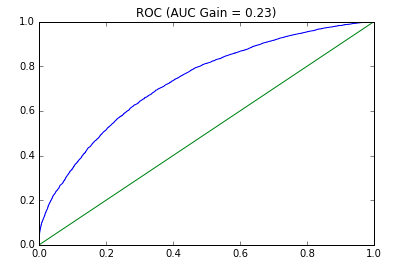
\includegraphics[scale=0.55]{ROC_rf} 
		\caption{\textbf{ Random forest classifier ROC with AUC Gain=0.23 }}
	\end{figure}
	
	
	\begin{figure}[H]
		%\hspace*{-1.85cm}
		\centering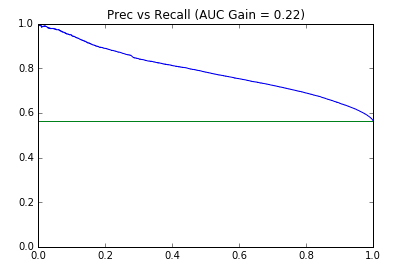
\includegraphics[scale=0.55]{prrc_rf} 
		\caption{\textbf{ Random forest classifer precision vs. recall with AUC Gain=0.22 }}
	\end{figure}
	
		\subsection{Quadratic Discriminant Analysis}
	QDA is a Bayesian classifier. Training and test accuracies were better than the baseline random forest but not as high as the multilayer perceptron classifier. 
	\begin{table}[h!]
		\begin{center}
			\caption{word2vec + Quadratic Discriminant Analysis}
			\label{tab:table1}
			\begin{tabular}{l|c|r} % <-- Alignments: 1st column left, 2nd middle and 3rd right, with vertical lines in between
				\textbf{Type} & \textbf{Training Set} & \textbf{Test Set}\\
				\hline
				Accuracy & 0.719376196853 & 0.71173456698 \\
				Precision & 0.769485042382 & 0.760003838403 \\
				Recall & 0.720252828854  & 0.706260032103\\
				F1 score & 0.744055433157 & 0.732146984054
			\end{tabular}
		\end{center}
	\end{table}
	
	\begin{figure}[H]
		%\hspace*{-1.85cm}
		\centering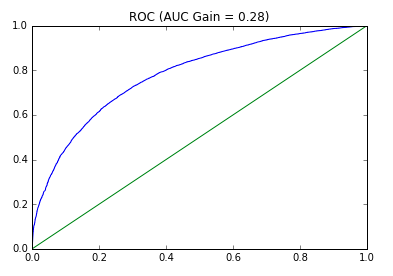
\includegraphics[scale=0.55]{ROC_qda} 
		\caption{\textbf{QDA classifier ROC with AUC gain=0.28 }}
	\end{figure}
	
	
	\begin{figure}[H]
		%\hspace*{-1.85cm}
		\centering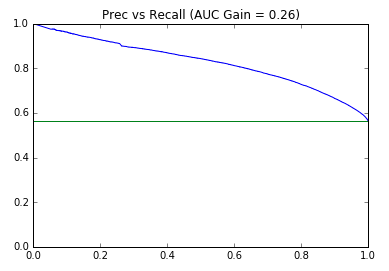
\includegraphics[scale=0.55]{prrc_qda} 
		\caption{\textbf{ QDA classifier precision vs. recall with AUC Gain=0.26 }}
	\end{figure}


	\subsection{Multi-Layer Perceptron}
	MLP yielded better accuracy on both training and test sets compared to random forest:
	\begin{table}[h!]
		\begin{center}
			\caption{word2vec + MultiLayer Perceptron (MLP)}
			\label{tab:table1}
			\begin{tabular}{l|c|r} % <-- Alignments: 1st column left, 2nd middle and 3rd right, with vertical lines in between
				\textbf{Type} & \textbf{Training Set} & \textbf{Test Set}\\
				\hline
				Accuracy & 0.811256993379 & 0.742028552952 \\
				Precision & 0.828856719281 & 0.765130190007 \\
				Recall & 0.840213932107  & 0.775637595862\\
				F1 score & 0.834496685544 & 0.77034806483
			\end{tabular}
		\end{center}
	\end{table}
	
	
	\begin{figure}[H]
		%\hspace*{-1.85cm}
		\centering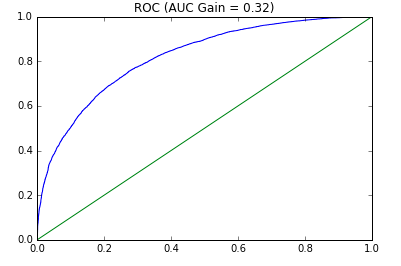
\includegraphics[scale=0.55]{ROC_nn} 
		\caption{\textbf{ MLP classifier ROC with AUC gain=0.32 }}
	\end{figure}
	

	
	\begin{figure}[H]
		%\hspace*{-1.85cm}
		\centering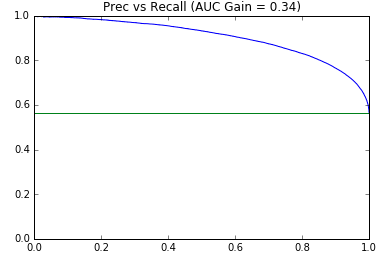
\includegraphics[scale=0.55]{prrc_nn} 
		\caption{\textbf{MLP classifier precision vs. recall with AUC Gain=0.34 }}
	\end{figure}
	
	MLP is simpler architecturally than the LSTM (discussed later), but it is a good choice of classifier because its training time is significantly lower than LSTM.
		

	
	
	\subsection{LSTM}
	The LSTM has a notion of memory. Its memory cell consists of four main elements: an input gate, a neuron with a path back to itself, a forget gate, and an output gate. The loop back allows the state of a memory cell to remain constant through time. The forget gate modulates the loop back and can allow the cell to "delete" or "forget" its previous state. LSTMs do not suffer from the vanishing or exploding gradient problem when long sequences are processed. It is an effective model for data that exhibits long-chain dependencies.  
	\subsubsection{LSTM Architecture}
	\begin{figure}[H]
		%	\hspace*{-1.3cm}
		\centering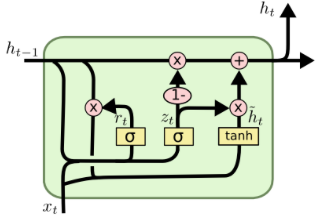
\includegraphics[scale=0.5]{lstm_image} 
		\caption{\textbf{ LSTM architecture.}}
	\end{figure}
	
	The figure above shows the basic LSTM architecture, including the notion of time (t-1 is introduced) and the gates previously discussed. Corresponding functions are shown below.
	\begin{figure}[H]
		%	\hspace*{-1.3cm}
		\centering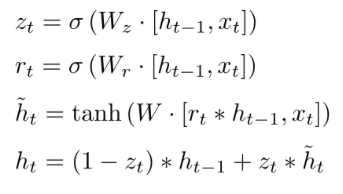
\includegraphics[scale=0.5]{lstm_functions} 
		\caption{\textbf{ LSTM functions.}}
	\end{figure}
	
	Our specific LSTM network's architecture consists of three layers. Words will be fed into the word embedding layer, which will map words to word embeddings. The resulting word vectors are passed into LSTM cells, whose output will be passed into a dense layer with softmax activation function, and makes a prediction. The high level view of data flow is shown in the implementation architecture in the figure below:
	
	\begin{figure}[H]
		%	\hspace*{-1.3cm}
		\centering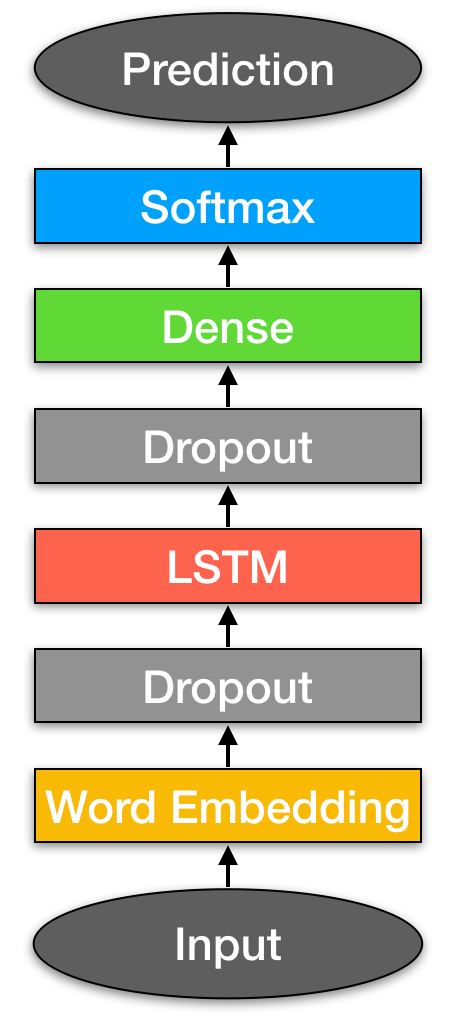
\includegraphics[scale=0.3]{architecture} 
		\caption{\textbf{ LSTM implementation architecture.}}
	\end{figure}
	
	\subsubsection{LSTM Implementation}
	Our LSTM model is implemented with Keras, running on top of TensorFlow. Keras is a high-level neural network API, which allowed us to quickly implement the model by simply stacking layers together:
	{\tt \small
		\begin{verbatim}
		model = Sequential()
		model.add(Embedding(...))
		model.add(Dropout(...))
		model.add(LSTM(...))
		model.add(Dense(..., activation='softmax'))
		\end{verbatim}
	}
	
	Our work largely follows Peter Nagy's implementation\cite{peter}, but we modified the network and tuned hyperparameters to suit our needs. Training the model took two hours to finish.
	
	\subsubsection{LSTM Results}
	The model achieves an F1-score of 0.81 and an Accuracy of 0.81 on test datasets, outperforming the MLP's F1-score of 0.77 and accuracy of 0.74.  \\
	%TODO verify max classifier performance
	
	\begin{center}
		\begin{tabular}{|c|c|}
			
			\hline
			Metrics & Value \\
			\hline
			Accuracy & 0.810448419184 \\
			Precision & 0.803874201171 \\
			Recall & 0.822235970902 \\
			F1-score & 0.812951416989 \\
			\hline
		\end{tabular}
	\end{center}
	
	While the results are good, the fact that the LSTM took so long to train made it a difficult model to use given our computational setup. With a real ML-machine or access to a set of GPUs in the cloud, we would have been able to more easily integrate it into the flow.
	\subsection{Hyperparameter Tuning}
	The hyperparameter tuning targets the hyperparameters of the word2vec model. Cross-validation was used on the original dataset. Since the MLP classifier had the best performance during the sentiment analysis evaluation phase, we chose to use this is the go-to classifier and invariant pairing. The F1-score of the word2vec + MLP classifier is used as a performance metric. Higher F1 score indicates a better performance. 
	\subsubsection{Testing Methodology}
	Word2vec turns text messages into word vectors. However, there is no systematic metric for the evaluation of the model alone. Therefore, evaluation of the bundle: Word2vec + MLP, was used to test the performance. \par
	The default method for hyperparameter tuning is to use an exhaustive grid search. However, since a single run of the 5-fold cross validation takes around 50 minutes, and some hyperparameters, such as size and iter, change the amount of work to be done, a brute force method would be too time consuming. Therefore hyperparameter selection and candidate selection was used. In the selection part, several hyperparameters are examined and the relatively important ones are picked. The resulting candidates for the tuning are:
	\begin{itemize}
		\item Size, which determines the dimensionality of the feature vector.
		\item \texttt{wind\_size}, the maximum distance between current and predicted words within a sentence, governs the context of words.
		\item \texttt{min\_count}, which defines the cut-off threshold for words.
		\item iter, number of iterations over the corpus.
	\end{itemize}
	The candidates for size is picked in the range from the default 100 to 150, \texttt{wind\_size} is picked from 1 to 10, which includes its default value 5. \texttt{min\_count} and iter are similar to the \texttt{wind\_size}. 
	\par
	This means a 2-D grid search could take around 3000 testing instances, which is impossible to handle. Therefore, 1-D search was performed on each hyperparameter, and a final search in the potential best candidate's neighborhood was conducted.
	\par
	The final candidates were further reduced based on their the neighbor's frequency in the 1-D search. If one of the two neighbors in the 1-D case has significantly lower score, it is omitted. Furthermore, size values are limited to only multiple of 4 to improve performance.
	
	\subsubsection{Testing Results}
	The following table summaries the 1-D search and the resulting search. \\
	%\hspace{-1cm}
	\begin{tabular}{|c|c|c|c|}
		\hline 
		hyperparameter & optimum F1 & best value & candidate \\
		\hline 
		\texttt{wind\_size} &  0.6286 & 1 & 1,4\\ 
		\hline 
		size & 0.657 & 130, 140  & 132, 140 \\
		\hline 
		\texttt{min\_count} & 0.6026 & 7 & 7,8 \\
		\hline 
		iter & 0.6101 & 9 & 9, 10 \\
		\hline 
	\end{tabular}
\\
\\
	The neighborhood search in the end gives the best candidates for hyperparameters: (140,1,7,9), (140,1,8,9), (140,1,8,10), and (140,4,8,10).
	
	\section{Stock Prediction} 
As mentioned earlier, because of a paucity of labeled sentiment data, we did not extend our sentiment analysis work to handle twitter data scraped using the API.  Instead, we decided to use historical stock prices as proxy labels for archived tweets.  Because we did not want to introduce another evaluation metric for models, preventing us from comparing stock prediction to sentiment prediction, we decided to perform classification on stock prices instead of regression. 
\par
To generate our (feature vector, label) tuples, we grouped tweets by company and date.  We selected opening stock prices for each company for each day and compared then to the opening price of the stock the next day to generate binary label.  For tweets, we reduced the resultant 2D array of word vectors with a multi dimensional average to generate a vector for each stock in our word embedding space.  We did not test more elaborate methods of composing word vectors into stock vectors, in future work, we could use the method of "document" embedding described in https://arxiv.org/abs/1405.4053.  The authors of this paper augment the standard context vector used as input for the simulated neural net of word2vec by adding an additional vector that describes which "document" (in our case this vector would map to a stock on a specific day) the context vector came from.
\par
We then applied the same battery of evaluation metrics to this dataset as for our sentiment analysis dataset. We split the data using an 80/20 training-testing division and then feed it to the MLP model. The default sklearn model was used, which includes only one hidden layer with 100 nodes. Other parameters are:  activation='relu', solver='adam', alpha=0.0001, batch\_size='auto', learning\_rate='constant', learning\_rate\_init=0.001, power\_t=0.5, max\_iter=200, shuffle=True, random\_state=None, tol=0.0001, verbose=False, warm\_start=False, momentum=0.9, nesterovs\_momentum=True, early\_stopping=False, validation\_fraction=0.1, beta\_1=0.9, beta\_2=0.999, epsilon=1e-08

\begin{table}[H]
	\centering
	\caption{Performance Metrics for MLP stock prediction}
	\label{my-label}
	\begin{tabular}{@{}lll@{}}
		\toprule
		\textbf{Metric} & \textbf{Train Set} & \textbf{Test Set} \\ \midrule
		F1-Score        & 0.7862                 & 0.7477                \\
		Precision       & 0.7481                 & 0.7102                \\
		Recall          & 0.8285                 & 0.7894                \\
		Accuracy        & 0.7458                 & 0.7001                \\ \bottomrule
	\end{tabular}
\end{table}

\begin{figure}[H]
	%	\hspace*{-1.3cm}
	\centering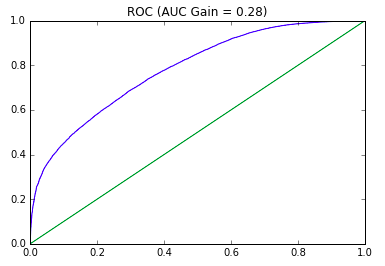
\includegraphics[scale=0.6]{mlp1} 
	\caption{\textbf{ROC curve for the MLP stock predictor model.}}
\end{figure}

\begin{figure}[H]
	%	\hspace*{-1.3cm}
	\centering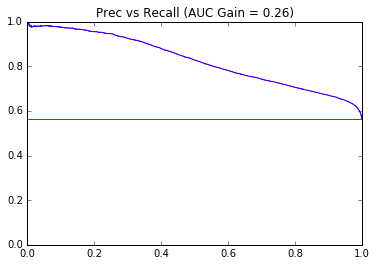
\includegraphics[scale=0.6]{mlp2} 
	\caption{\textbf{Precision vs. Recall curve for the MLP stock predictor model.}}
\end{figure}

	
By comparing the (F1,Accuracy,Precision,Recall) 4-ples for training and test sets we see there is some overfitting, but we can see the model extrapolates meaningfully to the test dataset by comparing the ROC and Precision/Recall curves (in blue) of our MLP classifier with the random classifier (where decisions are made solely on a biased coin flip, in green).  Note that the ROC and Precision/Recall curves were generated with test set data only.


\section{Conclusion}
Our performance, as indicated by F1-score, precision, recall, and accuracy, was reasonably high for the stock prediction class. Our F1-score of 0.7477 on the test set  significantly outperformed the random classifier. We chose MLP over the LSTM due to the faster training time, but given more time we would have liked to integrate the LSTM into the stock prediction pipeline rather than having it exist as just an exploratory design.
	\subsection{Future Work}
	Due to time limitations, we were not able to integrate the trained LSTM model with the rest of our functional blocks. However, our design was pipelined such that blocks (preprocessor, embedding scheme, sentiment analysis, and prediction) can be easily interchanged. Apart from adding in the LSTM, we would like to investigate other word embedding methods (such as GloVe), as well as other text-to-vector summarization methods. 
	\par
	Since the LSTM model showed a lot of promise, some future work that could be done on it would be to add attention, since a tweet's core meaning is generally encapsulated in a subset of the words rather than in the whole sequence itself. 
	
	\subsection{Task Distribution}
	Our work breakdown is summarized in the table below. Jonathan was responsible for performing the data crawling, preliminary data filtering, and writing the report. Amal preprocessed the crawled data and tested various models for sentiment analysis using the aforementioned performance metrics. Then, he performed the stock prediction/classification task. Jerry performed exploratory work by testing the RNN-based LSTM on the sentiment analysis corpus. Fred performed hyperparameter tuning.
\begin{table}[H]
	\centering
	\caption{Distribution of Work}
	\label{my-label}
	\begin{tabular}{@{}ll@{}}
		\toprule
		\textbf{Task}                                                                                 & \textbf{Owner}   \\ \midrule
		\begin{tabular}[c]{@{}l@{}}Data crawling, parsing,\\ data filtering\end{tabular}              & Jonathan Hurwitz \\
		\begin{tabular}[c]{@{}l@{}}Preprocessing, sentiment\\ analysis, stock prediction\end{tabular} & Amal Duriseti    \\
		\begin{tabular}[c]{@{}l@{}}Sentiment analysis with \\ RNN-based models\end{tabular}           & Jerry Chen       \\
		Hyperparameter tuning                                                                         & Fred Xu          \\ \midrule
		Writing Report                                                                                & Jonathan Hurwitz \\ \bottomrule
	\end{tabular}
\end{table}
	% include your own bib file like this:
	%\bibliographystyle{acl}
	%\bibliography{acl2017}
	%\nocite{*}
	%\bibliography{fr_bib}
	%\bibliographystyle{acl_natbib}
	
	
\section{References}
\begin{enumerate}
	\item Johan Bollen et al., Twitter mood predicts the stock market, Arxiv, 2010
	\item Tomas Mikolov, Kai Chen, Greg Corrado, and Jeffrey Dean. Efficient Estimation of Word Representations in Vector Space. In Proceedings of Workshop at ICLR, 2013
	\item Tomas Mikolov, Ilya Sutskever, Kai Chen, Greg Corrado, and Jeffrey Dean. Distributed Representations of Words and Phrases and their Compositionality. In Proceedings of NIPS, 2013
	\item Quoc Le and Tomas Mikolov. Distributed Representations of Sentences and Documents
\end{enumerate}




	%\appendix
	
	
	
\end{document}

